\clearpage
\section{Allocation of Failure Probability}\label{appendix:significance_allocation}
\cref{algorithm:conditional_composition} provides a dominating pair for a single step $n$ that is valid on the success set $A^{(n)}$ with failure probability $\Pr(\overline{A}^{(n)}) \le \beta^{(n)}$. To apply \cref{lemma:conditional_composition} to the entire mechanism, we need a global failure probability $\delta_E = \Pr(\cup_{n=1}^N \overline{A}^{(n)})$ covering all $N$ steps. 

Two standard strategies would be:
\begin{itemize}[noitemsep]
    \item \textbf{Union Bound:} We apply a union bound and distribute the failure budget across iterations such that $\sum_{n=1}^N \beta^{(n)} \le \delta_E$. In particular, we could use $\beta^{(n)} = \delta_E \mathbin{/} N$.
    Combined with the union bound across components $1 < i \leq b$, this leads to a per-bound significance of $\delta_E   \mathbin{/} (N \cdot (b-1))$.
    \item \textbf{Global Max Bound:} Rather than deriving a separate upper tail bound $\overline{\lambda_i}^{(n)}$ on the conditional reverse hazard $p(z = i \mid z \leq i, \vy_{1:n-1})$ within each step $n$ and for each component $i$, we instead compute a tail bound on
    $\max_{n \in [N]} p(z = i \mid z \leq i, \vy_{1:n-1})$. In particular, we can simply compute independent
    tail bounds and then use $\overline{\lambda_i} = \max_{n \in [N]} \overline{\lambda_i}^{(n)}$ across all steps.
    Combined with the union bound across components $1 < i \leq b$, this leads to a per-bound significance of $\delta_E   \mathbin{/} (b-1)$.
\end{itemize}

However, we observed across various matrix factorizations (see, e.g.,~\cref{fig:experiment_variational_family}) that the reverse hazard bounds
gradually increase within the first epoch, are almost constant within each subsequent epoch, and undergo large jumps in between epochs.
We therefore adopt a \textbf{hybrid strategy}:
We first distribute the failure probability $\delta_E$ via a union bound across epochs, i.e., overall budget $\delta_E \mathbin{/} k$ per epoch. Then, 
\begin{itemize}
    \item For the first epoch, we use a union bound, i.e., significance $\delta_E \mathbin{/} (k \cdot b \cdot (b-1)) = \delta_E \mathbin{/} (N \cdot (b-1))$ per bound.
    \item Within each subsequent epoch, we use a max bound across steps, i.e., significance $\delta_E \mathbin{/} (k \cdot (b-1))$ per bound. 
\end{itemize}
Note that the factor $(b-1)$ is from needing to take a union bound over all mixture components $1 < i \leq b$.
This approach is less conservative than a global max  bound while maintaining a higher significance of $\delta_E \mathbin{/} (k \cdot (b-1))$ for later tail bounds compared to the full  union bound.

\cref{fig:experiment_union_vs_max_bound} illustrates the effect of the different allocation strategies for multi-epoch DP-SGD and BSR($p=4$) with low ($\sigma=2$) and high ($\sigma=5$) noise levels.
The proposed hybrid strategy is optimal, across most steps, and only marginally beaten by the global max bound in the last epoch.
This confirms our design choice of allocating failure probability in a non-uniform manner.

\begin{figure}[h!]
    \centering

    \begin{subfigure}[t]{0.45\linewidth}
        \centering
        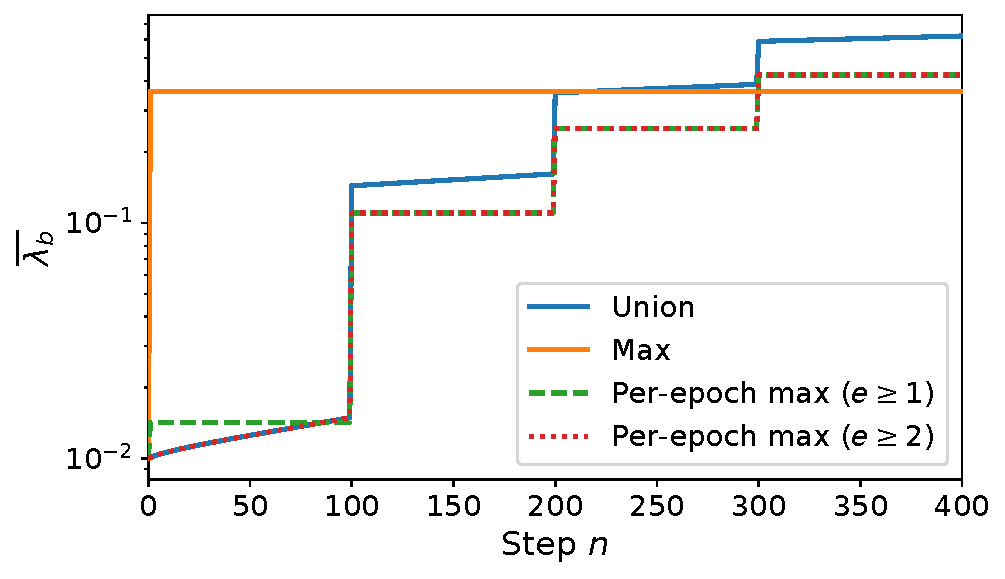
\includegraphics[width=\linewidth]{figures/union_vs_max_bound/dpsgd_4_epochs_100_batches_std_2.pdf}
        \subcaption{DP-SGD, $N=400,\ k=4,\ p=4,\ \sigma=2$}
    \end{subfigure}\hfill
    \begin{subfigure}[t]{0.45\linewidth}
        \centering
        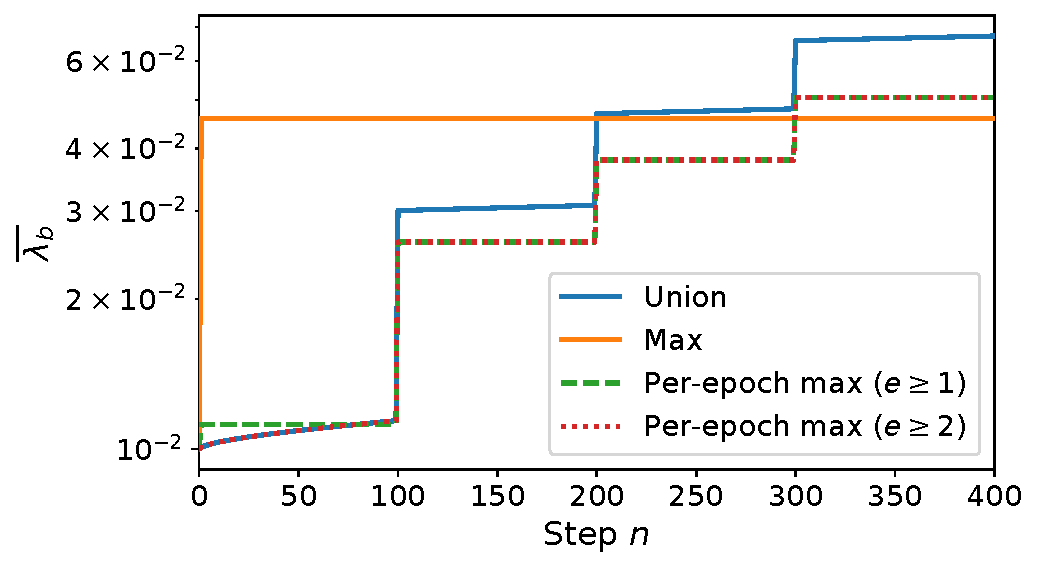
\includegraphics[width=\linewidth]{figures/union_vs_max_bound/dpsgd_4_epochs_100_batches_std_5.pdf}
        \subcaption{DP-SGD, $N=400,\ k=4,\ p=4,\ \sigma=5$}
    \end{subfigure}\hfill
    
    \begin{subfigure}[t]{0.45\linewidth}
        \centering
        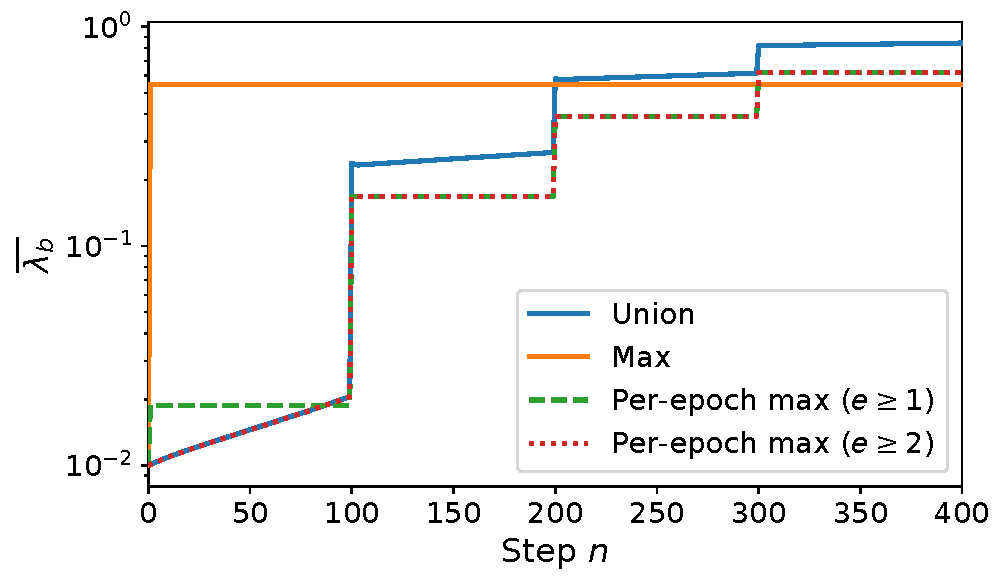
\includegraphics[width=\linewidth]{figures/union_vs_max_bound/bsr_4_epochs_100_batches_std_2.pdf}
        \subcaption{BSR, $N=400,\ k=4,\ p=4,\ \sigma=2$}
    \end{subfigure}\hfill
    \begin{subfigure}[t]{0.45\linewidth}
        \centering
        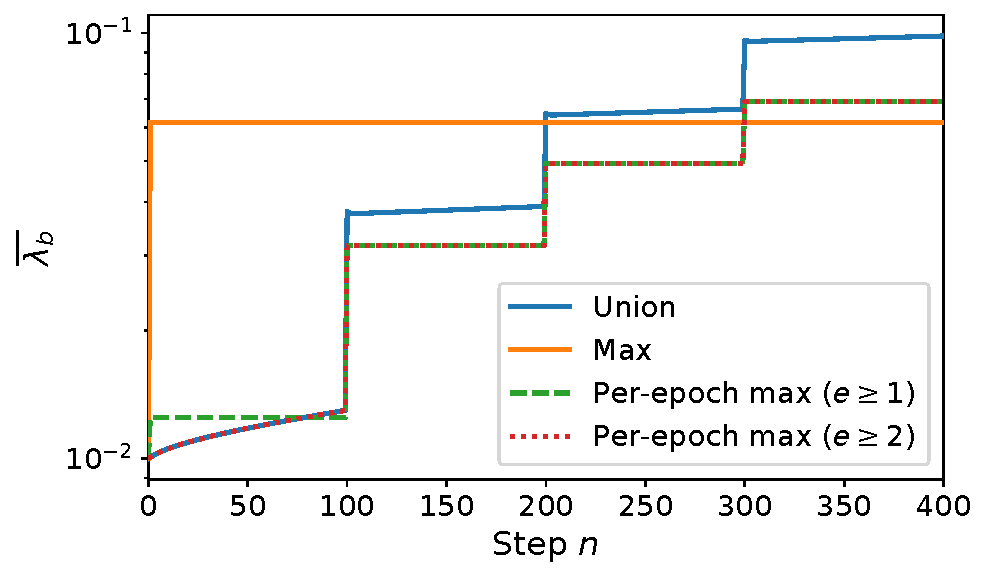
\includegraphics[width=\linewidth]{figures/union_vs_max_bound/bsr_4_epochs_100_batches_std_5.pdf}
        \subcaption{BSR, $N=400,\ k=4,\ p=4,\ \sigma=5$}
    \end{subfigure}\hfill
    \caption{Comparison of the largest mixture component's posterior probability $\overline{\lambda_b}$  (smaller is better)
    between different allocations of failure probability
    for different factorizations and noise multipliers $\sigma$ under $\delta_E = \SI{0.5e-5}{}$ and the ``remove'' relation.
    Using a union bound for the first epoch and a max bound for subsequent epochs (``Per-epoch max ($e \geq 2$)) performs best across most steps.
    Also using a max bound for the first epoch (``Per-epoch max ($e\geq 1$)) is only marginally better in the last few steps of the first epoch.
    Using a max bound across all steps (``Max'') is only marginally better in the last epoch and sacrifices the low subsampling rate $\overline{\lambda_b}$ of the first epoch's conditional composition dominating pairs.}
    \label{fig:experiment_union_vs_max_bound}
\end{figure}
\begin{figure}[h!]
    \centering

    \begin{subfigure}[t]{0.3\linewidth}
        \centering
        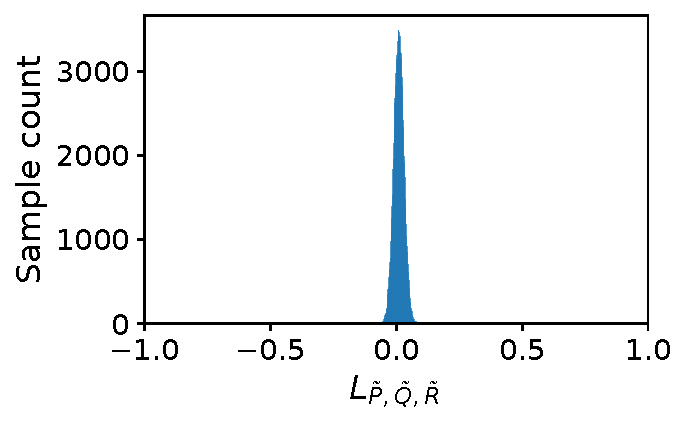
\includegraphics[width=\linewidth]{figures/posterior_jumps/dpsgd_4_epochs_100_batches_std_5.0_step_100.pdf}
        \subcaption{Step $100$}
    \end{subfigure}\hfill
    \begin{subfigure}[t]{0.3\linewidth}
        \centering
        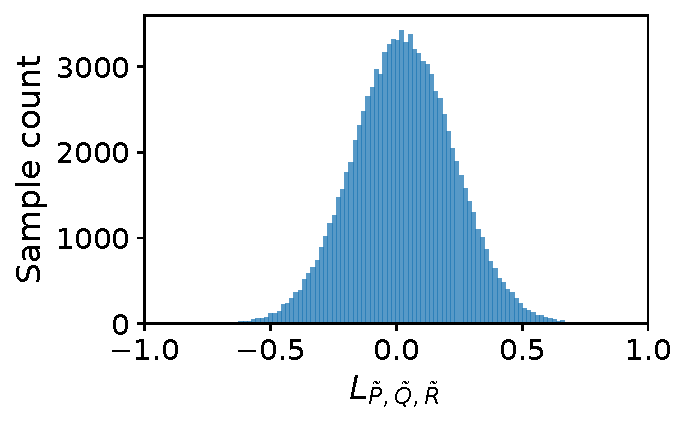
\includegraphics[width=\linewidth]{figures/posterior_jumps/dpsgd_4_epochs_100_batches_std_5.0_step_200.pdf}
        \subcaption{Step $200$}
    \end{subfigure}\hfill
    \begin{subfigure}[t]{0.3\linewidth}
        \centering
        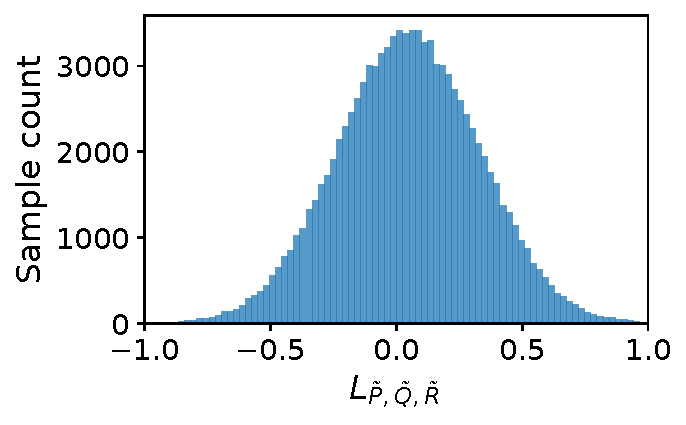
\includegraphics[width=\linewidth]{figures/posterior_jumps/dpsgd_4_epochs_100_batches_std_5.0_step_300.pdf}
        \subcaption{Step $300$}
    \end{subfigure}
    
    \begin{subfigure}[t]{0.3\linewidth}
        \centering
        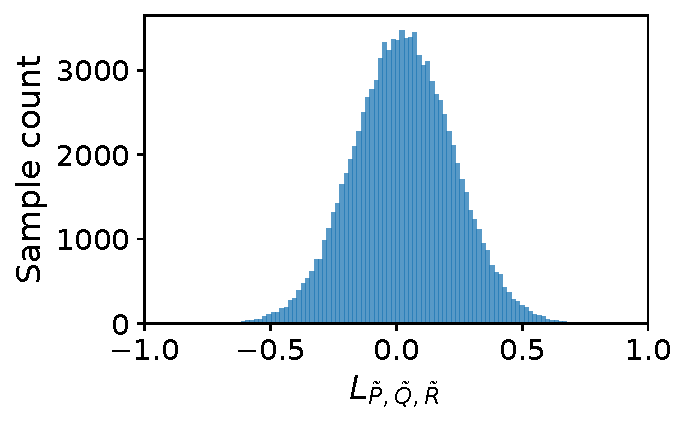
\includegraphics[width=\linewidth]{figures/posterior_jumps/dpsgd_4_epochs_100_batches_std_5.0_step_101.pdf}
        \subcaption{Step $101$}
    \end{subfigure}\hfill
    \begin{subfigure}[t]{0.3\linewidth}
        \centering
        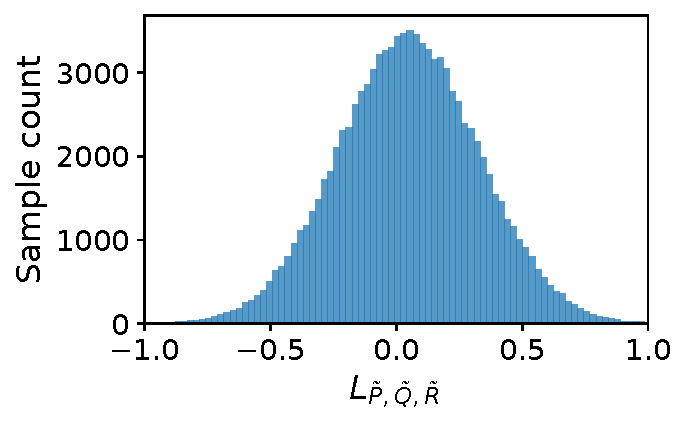
\includegraphics[width=\linewidth]{figures/posterior_jumps/dpsgd_4_epochs_100_batches_std_5.0_step_201.pdf}
        \subcaption{Step $201$}
    \end{subfigure}\hfill
    \begin{subfigure}[t]{0.3\linewidth}
        \centering
        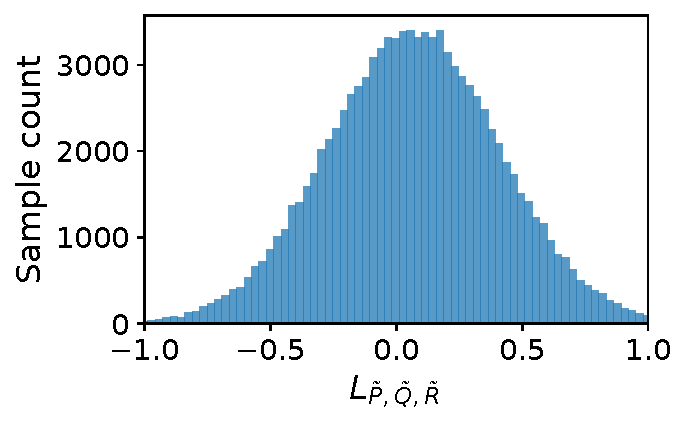
\includegraphics[width=\linewidth]{figures/posterior_jumps/dpsgd_4_epochs_100_batches_std_5.0_step_301.pdf}
        \subcaption{Step $301$}
    \end{subfigure}

    \caption{Sample histogram of the ternary privacy loss $L_{\tilde{P},\tilde{Q},\tilde{R}}$, whose lower tail is used to find reverse hazard upper bound $\overline{\lambda_b}$, shown at transitions between epochs.
    Samples are taken for DP-SGD with $k=4$ epochs, $b=100$ batches per epoch, and noise multiplier $\sigma=5$ for the ``remove'' relation.
    The histogram widens between epochs, which explains observed jumps in the reverse hazard bound.}
    \label{fig:posterior_jumps}
\end{figure}

\subsection{Remark on Jumps in Reverse Hazard}
At first, the jumps in our reverse hazard upper bound, which can be observed in both~\cref{fig:experiment_union_vs_max_bound} and~\cref{fig:experiment_variational_family} may seem abnormal or like an implementation error.
However, this is not the case. As an example, consider DP-SGD with $k$ epochs, $b$ batches per epoch, and $N = k \cdot b$ iterations overall. From the definition of our dominating pair in~\cref{lem:dominating_pair}, we know that the mixture means $\mm \in \sR^{k \cdot N}$ are simply
\begin{equation*}
    \mm = \begin{bmatrix}
        \eye_{b}\\
        \eye_{b}\\
        \cdots\\
        \eye_{b}
    \end{bmatrix},
\end{equation*}
i.e., a vertical stack of identity matrices, each with shape $b \times b$.
Consider an arbitrary step $n \in [N]$.
Recall from~\cref{algorithm:conditional_composition} that, to find our bound $\overline{\lambda_b}$ on the reverse hazard of the largest mixture component, we derive a lower tail bound on the ternary privacy loss $L_{\tilde{P}, \tilde{Q},\tilde{R}} = \log\left(\frac{\dd \tilde{P}}{\tilde{Q}}\right)(\vx)$ with $\vx \sim \tilde{R}$. Here, $\tilde{P}$ is a uniform mixture with means $\vmu_1, \dots, \vmu_{b-1} \in \{0,1\}^{n-1}$ taken from $\mm_{:, 1:n-1}$.
The distribution $\tilde{Q}$ is a single Gaussian with mean $\vmu_b \in \{0,1\}^{n-1}$.
In epoch $e = (n \mod b) + 1$, the single mean $\vmu_b$ of $\tilde{Q}$ has $\max\{e-1, 0\}$ non-zero entries.
Similarly, each mean $\vmu_j$ of $\tilde{P}$ has either $e$ or $\max\{e-1,0\}$ non-zero entries in distinct dimensions.
Thus, the pairwise distance between $\vmu_i$ and any $\vmu_j$ fulfills
\begin{equation*}
    ||\vmu_j - \vmu_i||_2 \in \{\sqrt{2e-1}, \sqrt{2e-2}\}.
\end{equation*}
Thus, the privacy loss increases from epoch to epoch.
In~\cref{fig:posterior_jumps}, we empirically verify this effect by taking $\SI{100000}{}$ samples from $L_{\tilde{P}, \tilde{Q}, \tilde{R}}$
for DP-SGD at the end and start of each epoch for $k=4$, $b=100$, $\sigma=5$.
We observe that the sample histogram of the privacy loss distribution significantly widens when transitioning from one epoch to the next.


\clearpage

\iffalse
\section{Asymptotic Analysis of the Variational Privacy Loss Bounds}

While~\cref{thm:remove_tail_bound} and~\cref{thm:add_tail_bound} provide an exact way to compute tail bounds using the Gaussian CDF, they do not explicitly show how the tail bounds scale with the means $\mm_1,\dots, \mm_b \in \sR^{N}$ and the noise multiplier $\sigma \in \sR_+$ of the matrix mechanism's overall dominating pair from~\cref{lem:dominating_pair}.
In particular, it does not show how the failure probability $\beta_i$ for each step $n \in N$ and each mixture component $i \in [b]$ (recall~\cref{algorithm:conditional_composition})
scales with the prefixes $\vmu_1 = \mm_{1,:n-1}, \dots, \vmu_b = \mm_{b,:n-1}$
that are used to construct per-iteration dominating pair $P^{(n)},Q^{(n)}$.


To analyze the asymptotic behavior, we apply standard Gaussian concentration inequalities to the previously derived bounds. For simplicity, we focus on the ``add'' case (a similar result could be shown for the remove case by taking the maximum over all mixture components).
\begin{proposition}\label{prop:asymptotic_bound}
    Let $\underline{L_i}(\vx) \sim \mathcal{N}(\nu, \xi)$ be the variational privacy loss lower bound derived in \cref{thm:add_tail_bound}. For any threshold $\tau < \nu$, the tail probability is bounded by:
    \begin{equation}
        \Pr[L_i(\vx) \leq \tau] \leq \exp\left( - \frac{(\nu - \tau)^2}{2\xi^2} \right),
    \end{equation}
    with
    \begin{align*}
        \nu &= \frac{1}{2\sigma^2} \left( \|\vmu_i\|_2^2 - \mathbb{E}_{j \sim \psi^{(k)}}[\|\vmu_j\|_2^2] \right) - \mathrm{KL}(\psi \mid\mid \pi), \\
        \xi &= \frac{1}{\sigma} \| \vmu_i - \mathbb{E}_{j \sim \psi}[\vmu_j] \|_2.
    \end{align*}
\end{proposition}

\begin{proof}
    The random variable $L_i(\vx)$ follows a normal distribution with mean $\nu$ and standard deviation $\xi$. We standardize this variable to $Z = \frac{L_i(\vx) - \nu}{\xi}$, which follows $\mathcal{N}(0, 1)$.
    The event $L_i(\vx) \leq \tau$ is equivalent to $Z \leq \frac{\tau - \nu}{\xi}$. Defining $t = \frac{\nu - \tau}{\xi}$, the condition $\tau < \nu$ implies $t > 0$.
    Applying the standard Gaussian concentration inequality $\Pr[Z \leq -t] \leq e^{-t^2/2}$ and substituting $t$ yields the result.
\end{proof}

To interpret this bound, we analyze the case of a uniform variational distribution $\psi$.
There, the parameters simplify to $\nu = \frac{1}{\sigma^2} (\|\vmu_i\|_2^2 - \overline{\|\vmu\|_2^2})$ and $\xi = \frac{1}{\sigma} \|\vmu_i - \bar{\vmu}\|_2$,
with averages $\overline{\|\vmu\|_2^2} = \frac{1}{i-1} \sum_{j=1}^{i-1} ||\vmu_j||_2^2$ and  $\bar{\vmu} = \frac{1}{i-1} \sum_{j=1}^{i-1} \vmu_j$.
Substituting these into \cref{prop:asymptotic_bound} with $\tau=0$ yields an exponent of the form:
\begin{equation}
    \frac{\nu^2}{2\xi^2} = \frac{1}{8\sigma^2} \cdot \underbrace{\frac{ \left( \|\vmu_i\|_2^2 - \overline{\|\vmu\|_2^2} \right)^2 }{ \|\vmu_i - \bar{\vmu}\|_2^2 }}.
\end{equation}
Consequently, ...

\clearpage


\fi


\section{Choice of Variational Family}\label{appendix:choice_of_variational_family}
Recall from~\cref{algorithm:conditional_composition} that we need to find a lower tail bound on the ternary privacy loss  random variable $L_{\tilde{P}, \tilde{Q}, \tilde{R}}$,
which is defined as $L_i(\vx)$ with $L_i(\vx) = \log\left(\frac{\dd \tilde{P}}{\dd \tilde{Q}}\right)(\vx)$ and $\vx \sim \tilde{R}$,
where $\tilde{P}$ is a uniform Gaussian mixture with means $\vmu_1,\dots,\vmu_{i-1}$,
$\tilde{Q}$ is a single Gaussian with mean $\vmu_i$,
and $\tilde{R}$ is either:
\begin{itemize}
    \item $\sum_{k=i}^{b} \mathcal{N}(\mmu_k, \sigma^2 \eye_{n-1}) \cdot \frac{1}{b}$ (``remove'' case),
    \item or $\mathcal{N}(\vzero, \sigma^2 \eye_{n-1})$ (``add'' case), which is equivalent to the trivial mixture
    $\sum_{k=i}^{b} \mathcal{N}(\vzero, \sigma^2 \eye_{n-1}) \cdot \frac{1}{b}$.
\end{itemize}
Let $\vrho_k \in \sR^{n-1}$ denote an arbitrary component mean of $\tilde{R}$ (either $\vmu_k$ or the all-zeros vector $\vzero$).
From~\cref{lemma:variational_distribution_general,thm:remove_tail_bound,thm:add_tail_bound}, we know that the tail probability conditioned on component $k$ is upper-bounded via
\begin{equation}\label{eq:single_component_tail_bound}
    \Pr_{\vx \sim \mathcal{N}(\vrho_k, \sigma^2 \eye)}[L_i(\vx) \leq \tau] \leq \Phi\left( \frac{\tau - \nu_k}{\xi_k} \right)
\end{equation}
with scalar mean $\nu_k \in \sR$ and scalar standard deviation $\xi_k \in \sR_+$
with
\begin{align}
    \nu_k &= \frac{1}{\sigma^2} \vmu_k^T (\mathbb{E}_{j \sim \psi^{(k)}}[\vmu_j] - \vmu_i) + \frac{1}{2\sigma^2} \left( \|\vmu_i\|_2^2 - \mathbb{E}_{j \sim \psi^{(k)}}[\|\vmu_j\|_2^2] \right) - \mathrm{KL}(\psi^{(k)} \mid\mid \pi),
    \label{eq:variational_per_component_mean}
    \\
    \xi_k &= \frac{1}{\sigma} \| \vmu_i - \mathbb{E}_{j \sim \psi^{(k)}}[\vmu_j] \|_2,
    \label{eq:variational_per_component_std}
    \\
    \pi &= \mathrm{Uniform}(\{1,\dots,i-1\}),
\end{align}
for any variational distribution $\psi^{(k)}$ over mixture indices $\{1,\dots, i-1\}$.
Therefore, we can define an entire variational family $\Psi^{(k)}$ and choose a $\psi^{(k)} \in \Psi^{(k)}$ that leads to the tightest tail bound.

In principle, we could let $\Psi^{(k)}$ be the set of all distributions supported on $\{1,\dots, i-1\}$ and explicitly optimize $\psi^{(k)}$ (e.g., via gradient descent, which would be an interesting direction for future work).
However, for $k \in \sN$ epochs and $b \in \sN$ batches per epoch and thus $N = k \cdot b$, we would need to solve
$N \cdot b^2$ such optimization problems (one for each step $n$, each privacy loss $L_i$ with $i \in [b]$, and  each component $k \in [b]$ of $\tilde{R})$. 
We therefore consider the following heuristically chosen variational families instead:

\subsection{Option 1: Maximizing the expectation based on KL divergence}
A heuristic for tightening the bound in~\cref{eq:single_component_tail_bound}
is by maximizing the mean $\nu_k$.
In turn, a heuristic for doing so is to eliminate the  KL-divergence term in~\cref{eq:variational_per_component_mean}
by letting
\begin{equation*}
    \psi^{(k)} = \pi = \mathrm{Uniform}(\{1,\dots, i-1\}.
\end{equation*}
This corresponds to taking the geometric mean of privacy losses, which we already used in deriving our R\'enyi divergence bound from~\cref{lem:remove-renyi-bound}.

\subsection{Option 2: Maximizing the expectation based on component distance}
Another heuristic for maximizing the mean is to apply quadratic expansion, i.e., 
\begin{equation*}
    \nu_k = - \frac{1}{2 \sigma^2} \mathbb{E}_{j \sim \psi^{(k)}}\left[||\vrho_k - \vmu_j||_2^2\right]
    + \frac{||\vrho_k - \vmu_i||_2^2}{2\sigma^2} - \mathrm{KL}(\psi^{(k)} || \pi),
\end{equation*}
and notice that the second term does not depend on variational distribution $\psi^{(k)}$.
Instead of minimizing the KL-divergence, we could instead define $\psi^{(k)}$ to minimize the distance in the first term, i.e., $\psi^{(k)}(z=j) = 1 \iff j = \mathrm{argmin} ||\rho_k - \vmu_j||_2^2$.
To smoothly interpolate between this solution and minimization of the KL divergence, we can define
the variational family as
$\Psi^{(k)} = \{\psi(t, \vrho_k, (\vmu_1,\dots,\vmu_{i-1}\}) \mid t \in T\}$ with
\begin{equation*}
    \psi(t, \vrho_k, (\vmu_1,\dots,\vmu_{i-1})\}
    = \mathrm{softmax}\left( \left\{- \frac{||\vrho_k - \vmu_j||_2^2}{t } \middle| 1 \leq j < i\right\} \right)
\end{equation*}
for some fixed set of non-negative temperatures $T \subset \sR_+$.

\subsection{Option 3: Minimizing the standard deviation based on component distance}
Another heuristic for tightening the tail bound in~\cref{eq:single_component_tail_bound}
is by minimizing the standard deviation $\nu_k$, which makes the argument of Gaussian CDF $\Phi$ smaller for any $\tau \leq \nu_k$, i.e., any tail probability smaller than $0.5$.
Analogous to the previous approach, we can define
$\Psi^{(k)} = \{\psi(t, \vmu_i, (\vmu_1,\dots,\vmu_{i-1})\} \mid t \in T\}$ with
\begin{equation*}
    \psi(t, \vmu_i, (\vmu_1,\dots,\vmu_{i-1})\}
    = \mathrm{softmax}\left( \left\{- \frac{||\vmu_i - \vmu_j||_2^2}{t } \middle| 1 \leq j < i\right\} \right)
\end{equation*}
for some fixed set of non-negative temperatures $T \subset \sR_+$.
Notice that, unlike the previous approach, this variational family is independent of the component mean $\vrho_k$, i.e.,
we use the same variational family across all components of $\tilde{R}$.

\subsection{Our choice.}
In our experiments, we opt for Option 3, since it only requires evaluation of a linear number of distances $||\vmu_i - \vmu_j||$,
and this computational cost is shared across all $K$ components of our tail bound.
We additionally include $\tau = \infty$, which corresponds to the KL-minimizing uniform distribution from Option 1.
For our experiments, we specifically use temperatures $T = \{\infty\} \cup \{10^{-1}, 10^{-0.5}, 1, 10^{0.5}, 10^{1}\}$, which we found to improve tightness of our accountant compared to Option 1 ($T = \{\infty\}$) alone, i.e., the geometric mean.
Furthermore, we empirically did not find Option 2 to offer any increased tightness.
\cref{fig:experiment_variational_family} demonstrates this through an empirical comparison across different matrix factorizations and noise levels in the multi-epoch setting.

\begin{figure}[h]
    \centering

    \begin{subfigure}[t]{0.45\linewidth}
        \centering
        
\includegraphics[width=\linewidth]{figures/variational_family/bsr_4_epochs_100_batches_std_2.pdf}
        \subcaption{BSR, $N=400,\ k=4,\ p=4,\ \sigma=2$}
    \end{subfigure}\hfill
    \begin{subfigure}[t]{0.45\linewidth}
        \centering
        
\includegraphics[width=\linewidth]{figures/variational_family/bsr_4_epochs_100_batches_std_5.pdf}
        \subcaption{BSR, $N=400,\ k=4,\ p=4,\ \sigma=5$}
    \end{subfigure}\hfill
    
    \begin{subfigure}[t]{0.45\linewidth}
        \centering
        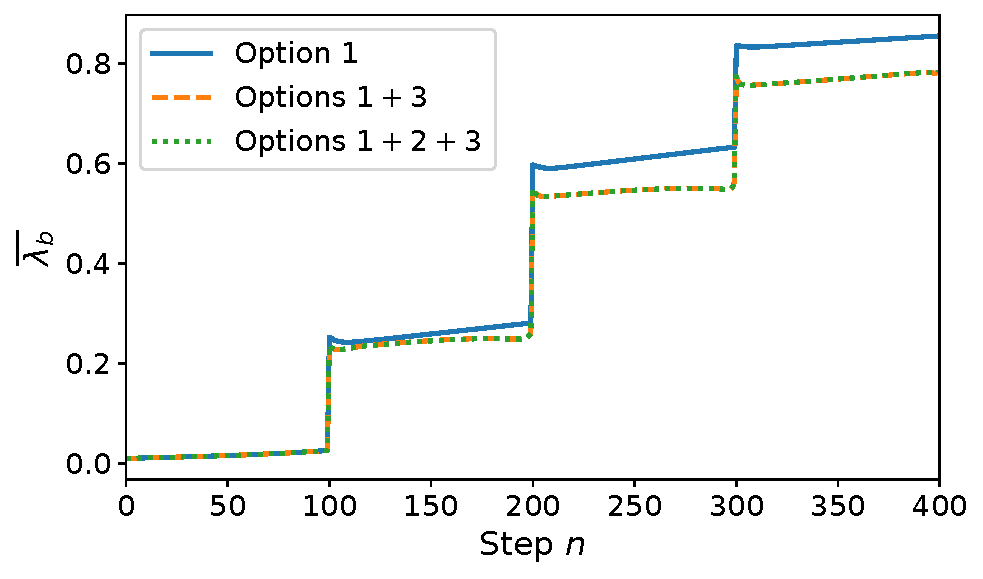
\includegraphics[width=\linewidth]{figures/variational_family/bisr_4_epochs_100_batches_std_2.pdf}
        \subcaption{BISR, $N=400,\ k=4,\ p=4,\ \sigma=2$}
    \end{subfigure}\hfill
    \begin{subfigure}[t]{0.45\linewidth}
        \centering
        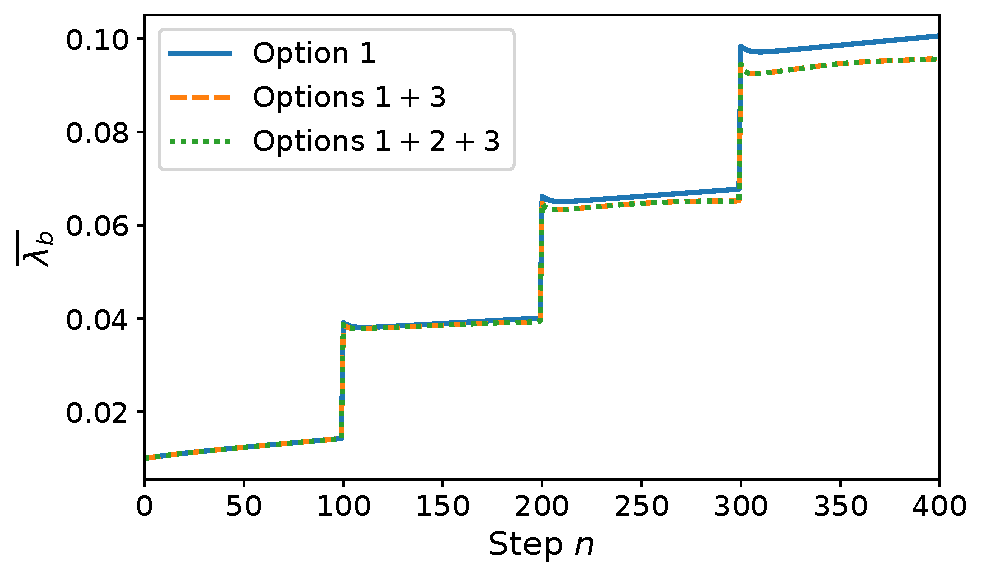
\includegraphics[width=\linewidth]{figures/variational_family/bisr_4_epochs_100_batches_std_5.pdf}
        \subcaption{BISR, $N=400,\ k=4,\ p=4,\ \sigma=5$}
    \end{subfigure}\hfill
    \caption{Comparison of the largest mixture component's posterior probability $\overline{\lambda_b}$  (smaller is better)
    between variational families 
    for different factorizations and noise multipliers $\sigma$ under $\delta_E = 10^{-5}$ and the ``remove'' relation.
    In later epochs, minimizing variance of the tail bound (``Options 1+3'') improves upon only taking the geometric mean 
    via a uniform distribution (``Option 1'').
    The effect is more pronounced in settings where  the noise multiplier is small and sensitivity is large ($\sigma=2$, BISR),
    compared to settings where the noise multiplier is large and the overall sensitivity is small ($\sigma=5$, BSR).
    Maximizing the mean (``Option 2'') does not further improve the posterior bound.
    }
    \label{fig:experiment_variational_family}
\end{figure}

\subsection{Overall Computational Cost of Tail Bounds}
In each step $n \in [N]$ and for each component $i \in [b]$, 
the cost of deriving the tail bound $\tau_i$ in~\cref{algorithm:conditional_composition} is dominated by computing distances $\|\boldsymbol{\mu}_i - \boldsymbol{\mu}_j\|^2$, each of which has a cost of $\mathcal{O}(n)$. A na\"ive implementation of re-computing these distances for vectors in $\mathbb{R}^n$ at every step and for each component leads to an overall complexity  of $\mathcal{O}(N^2 b^2)$.
We use this na\"ive approach in the implementation provided with the supplementary material.

However, to scale to larger $N$, one could in principle reduce the overall cost to $\mathcal{O}(N b^2)$ using incremental updates. By maintaining the Gram matrix of the mixture means $\vmu_1,\dots,\vmu_b$ starting from step $n=1$, one can exploit the prefix structure of the means: the inner products for step $n$ are simply those of step $n-1$ plus the product of the current batch contributions. This would allow for constant-time distance evaluation at each step after a $\mathcal{O}(b^2)$ update.

\clearpage

\section{Add and Remove Direction Dominating Pairs}\label{appendix:add_remove_flip}
Recall that we assume the following dominating pair:
\fulldominatingpair*
That is:
\begin{itemize}[nosep]
    \item In the ``remove'' case, $P$ is a Gaussian mixture and $Q$ is a single multivariate Gaussian.
    \item In the ``add'' case $P$ is a single Gaussian and $Q$ is a Gaussian mixture.
\end{itemize}
In the original Lemma 3.2 of~\cite{choquette2024near}, the directions are reversed. However, this appears to be a typing error.
Their proof for the ``add'' case actually argues correctly that the first argument of the hockey-stick divergence should be a zero-mean  Gaussian and the second argument should be a Gaussian mixture (note that in their proof $\vz$ is a zero-mean Gaussian):
``We give the proof for the \underline{add adjacency} [...]
Because each user is assigned to their batch independently, we can assume without loss of generality that contributions from all users other than the differing user are always $0$. In more detail, by post-processing, we can assume that we release the contributions to the input matrix of all examples except the differing user's. Let $\vx$ be these contributions, and $\vx'$ be $\vx$ plus the contribution of the differing user. Then distinguishing $\mC \vx + \vz$ and $\mC \vx' + \vz$ is equivalent to \underline{distinguishing $\vz$ and $\mC (\vx' - \vx) + \vz$} [ ...]``.

Further note that the same pattern of $P$ being a mixture under ``remove'' and $Q$ being a mixture under ``add'' arises in various other subsampling schemes, such as Poisson subsampling or subsampling without replacement (see, e.g., Theorem 11 in~\cite{zhu2022optimal}).